\documentclass{article}

\usepackage[utf8]{inputenc}
\usepackage[spanish]{babel}
\usepackage{amsthm}
\usepackage{nccmath}
\usepackage{enumitem}
\usepackage{graphicx}
\usepackage{verbatim}
\usepackage{algpseudocode}

\theoremstyle{plain}
\newtheorem{proposicion}{Proposición}

\theoremstyle{definition}
\newtheorem{definition}{Definición}[section]
\newtheorem{example}{Ejemplo}[section]

\title{Teoría de Autómatas y Lenguajes Formales\\[.4\baselineskip]Práctica 4.}
\author{Alejandro Rodríguez Moreno }
\date{Diciembre 2022}

\begin{document}

\maketitle

\section{Create the simplest WHILE program that computes the diverge function and compute the codification of its code. }

\begin{verbatim}
                     Q = (0,s)
                       s:
                         X1 := X1 + 1;
                         while X1 != 0 do
                          X1 := X1
                         od
\end{verbatim}
Consideramos la primera instruccion es la mas importante debido a que es la que nos asegura que el programa siempre diverje. La divergencia es producida al producirse un bucle infinito. 

\begin{center}
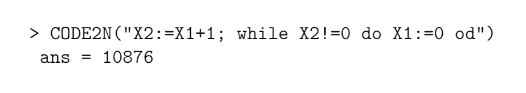
\includegraphics[width=9cm, height=2cm]{P4_E1.png}
\end{center}
\newpage

\section {Create an Octave script that enumerates all the vectors.}
\begin{verbatim}
function printNvectors(N)
    for i=0:N-1
    disp([’(’ num2str(godeldecoding(i)) ’)’])
    end
end
\end{verbatim}
Iteraremos sobre un número inicial 0, hasta un número deseado, mostrando el producto al aplicar godelcoding.


\section {Create an Octave script that enumerates all the WHILE programs.}
\begin{verbatim}
function printNwhilePrograms(N)
for i=0:N-1
disp(N2WHILE(i))
end
end
\end{verbatim}
Mismo esquema que el ejercicio anterior, no obstante en cada iteración de este ejercicio mostraremos el programa WHILE asociado al número correspondiente.


\end{document}
